% Deployment Integration Progress Report
\documentclass[12pt]{article}
\usepackage[margin=1in]{geometry}
\usepackage{graphicx}
\usepackage{caption}
\usepackage{float}
\usepackage[colorlinks=true, linkcolor=blue, urlcolor=blue]{hyperref}

\title{Deployment Integration Progress Report\\Deployment System}
\author{0104C}
\date{\today}

\begin{document}

\maketitle

\section{Introduction}

This report documents the integration process for the deployment mechanism, covering the step-by-step testing and troubleshooting of both servo subsystems. Integration involved combining the key servo (DF9GMS), the gear rack drive servo (MG996R), electrical wiring, and software control into a single functional deployment system.

\section{Integration Progress}

\subsection{Initial Key Servo Integration}

The first integration step connected the DF9GMS key servo to the deployment mechanism. As shown in \href{https://drive.google.com/file/d/1B9kVSxmLEpAjHLskNOtt1WgFnR0hwxYz/view?usp=drive_link}{Video 1}, the servo was operational but the control was poorly configured due to the servo speed being set too high in the code. As a result, the servo wiring began tangling during operation. Code recalibration was identified as a necessary next step.

\subsection{Key Lock Mechanism Verification}

Following successful code calibration, \href{https://drive.google.com/file/d/1NQgJGBopf075Fg2TIalUC3SOWtdoGTqC/view?usp=drive_link}{Video 2} demonstrates the key lock mechanism successfully attaching to the top of the sensor box. By actuating the key servo, the lid of the box was lifted, confirming successful integration of this subsystem.

\subsection{Gear Rack and Drive Servo Integration}

\href{https://drive.google.com/file/d/1bk9nI8Et9fE22TSZefOFPIE9JOT5nB2-/view?usp=drive_link}{Video 3} shows the integration of the gear rack with the MG996R servo motor. The rack was successfully driven up and down via push button control, consistent with the software design outlined in prototype 04.1.1. Both electrical and software components functioned as intended.

\subsection{Gear Rack Failure and Repair}

Shortly after the successful gear rack test, the rack broke and required regluing, as documented in \href{https://drive.google.com/file/d/1qpb2zd5Z0qnc0p-z-dHw--lwabcQHpc3/view?usp=drive_link}{Video 4}. This introduced a brief setback in the integration timeline but was resolved by reapplying adhesive to the joint.

\subsection{Servo Voltage Correction}

During integration, the DF9GMS key servo was found to be wired to the 5V output of the motor driver rather than the 3.3V source on the Pico board. This caused the servo to burn out. Three units were lost before the wiring error was identified and corrected. Figure \ref{fig:voltage_change} shows the rewired configuration after switching to the correct 3.3V supply.

\begin{figure}[H]
\centering
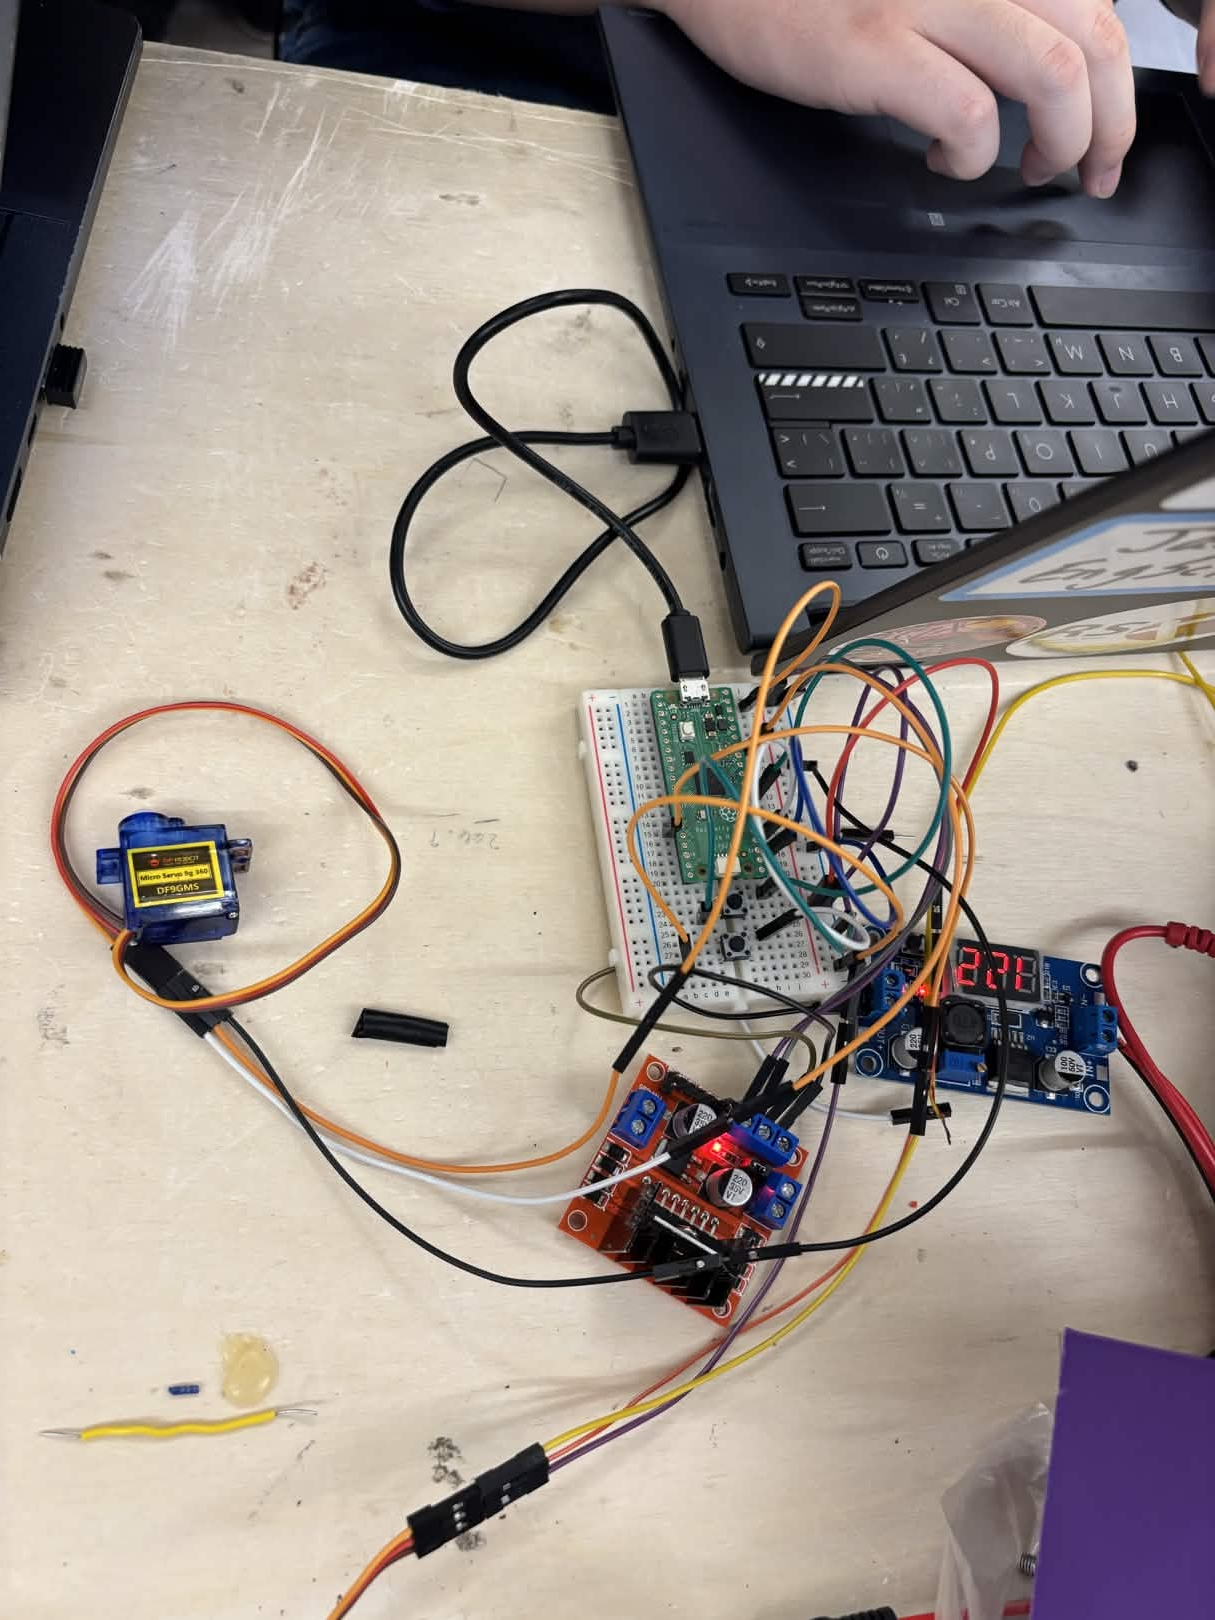
\includegraphics[width=0.65\textwidth]{9_Change of micro servo from 5 V to 3.3 V.jpg}
\caption{Key servo rewired from 5V motor driver output to 3.3V Pico board supply.}
\label{fig:voltage_change}
\end{figure}

\subsection{Final Dual-Servo Integration}

\href{https://drive.google.com/file/d/1d9S-s-2mgezRFPzDB1qaqtI1xFciR_Ff/view?usp=drive_link}{Video 6} shows both the DF9GMS and MG996R servos operating in unison under push button control. This confirms successful integration of both servo subsystems within the deployment mechanism. Full deployment demonstration, including integration with the sensor system, will be presented in 04.3.3.

\section{Conclusion}

Integration of the deployment mechanism was completed through an iterative process of testing, troubleshooting, and correction. Key issues encountered included improper servo speed configuration, a gear rack joint failure, and an incorrect voltage supply to the key servo. Each issue was resolved, resulting in both servos functioning correctly under coordinated push button control.

\end{document}
